\documentclass[main.tex]{subfiles}

\begin{document}
    \justifying

    \section{A domain-specific approach to scientific software development}
    \label{section:domain-specific-approach-to-scientific-software-development}

        In scientific software development, it is common practice to conceive a first proof-of-concepts implementation of a numerical algorithm in a high-level programming environment like MATLAB/Octave \citep{lindfield18}, or Python. Because these languages do not require compilation and support dynamic typing, they provide a breeding ground for fast prototyping. However, the direct adoption of interpreted languages in HPC has historically been hindered by their intrinsic slowness. To squeeze more performance out of the underlying silicon, the initial proof-of-concept is translated into either Fortran, C or C++. This leads to the so-called ``two-language problem'', where the programming language used for the germinal prototyping is abandoned in favor of a faster language that might be more complicated to use. The lower-level code can be parallelized for shared memory platforms using OpenMP directives, while distributed memory machines can be targeted using Message Passing Interface (MPI) libraries. % to handle data movements between remote memories.
        The resulting code can later be migrated to GPUs, offering outstanding compute throughput and memory bandwidth especially for Single Instruction Multiple Data (SIMD) applications. GPU porting is accomplished using either OpenACC or OpenMP directives, or via a CUDA\footnote{\url{https://docs.nvidia.com/cuda/}} or HIP\footnote{{https://rocm.docs.amd.com/projects/HIP/en/latest/}} rewriting, amongst others. To efficiently run the model at scale on multiple GPUs, a GPU-aware MPI build should be chosen, so to possibly avoid costly memory transfers between host and device and better overlap computations and communications.

        The schematic visualization in Fig.\,\ref{fig:dsl}a highlights how the above workflow leads to multiple implementations of the same scientific application utilizing different programming models and coding styles. This unavoidably complicates software maintainability: ideally, any modification in the numerical model should be encoded in all implementations, so to preserve the coherency across the hierarchy. The maintainability problem is exacerbated as the number of lines of code, the pool of platforms to support, and the user-base increase. This situation has been known as the ``software productivity gap'' \citep{lawrence18}, and we argue that it cannot be alleviated by relying on general-purpose programming paradigms and monolithic code designs. Instead, it calls for a more synergistic collaboration between domain scientists (which here include model developers, weather forecasters, and weather and climate scientists) and computer experts. A path forward is provided by DSLs through \emph{separation of concerns} (Fig.\,\ref{fig:dsl}b), so that domain scientists can express the science using syntactic constructs that are aligned with the semantics of the application domain and hide any architecture-specific detail. The resulting source code is thus hardware-agnostic, more concise, easier to read, and easier to manipulate. A toolchain developed by software engineers then employs automatic code generation techniques to synthesize optimized parallel code for the target computer architecture in a transparent fashion.

        \begin{figure}[t!]
            \centering

            \begin{minipage}{0.495\textwidth}
                \centering
                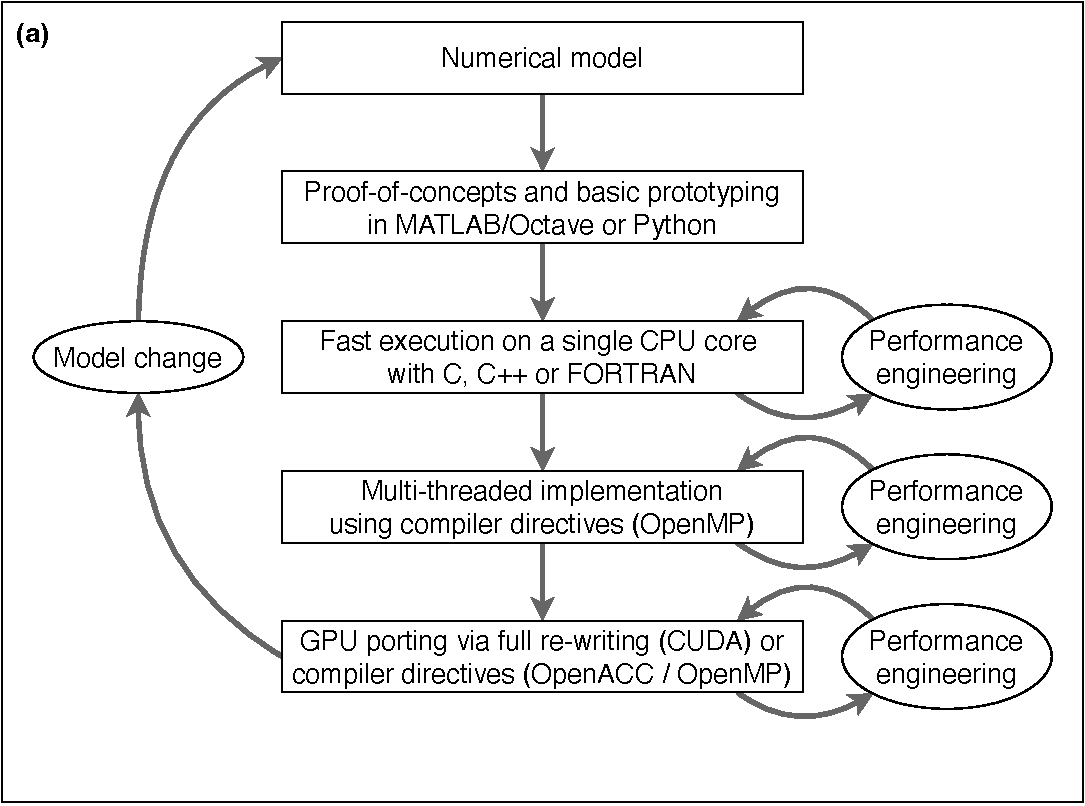
\includegraphics[scale=0.475]{workflow_2.pdf}
            \end{minipage}
            %\hfill
            \begin{minipage}{0.495\textwidth}
                \centering
                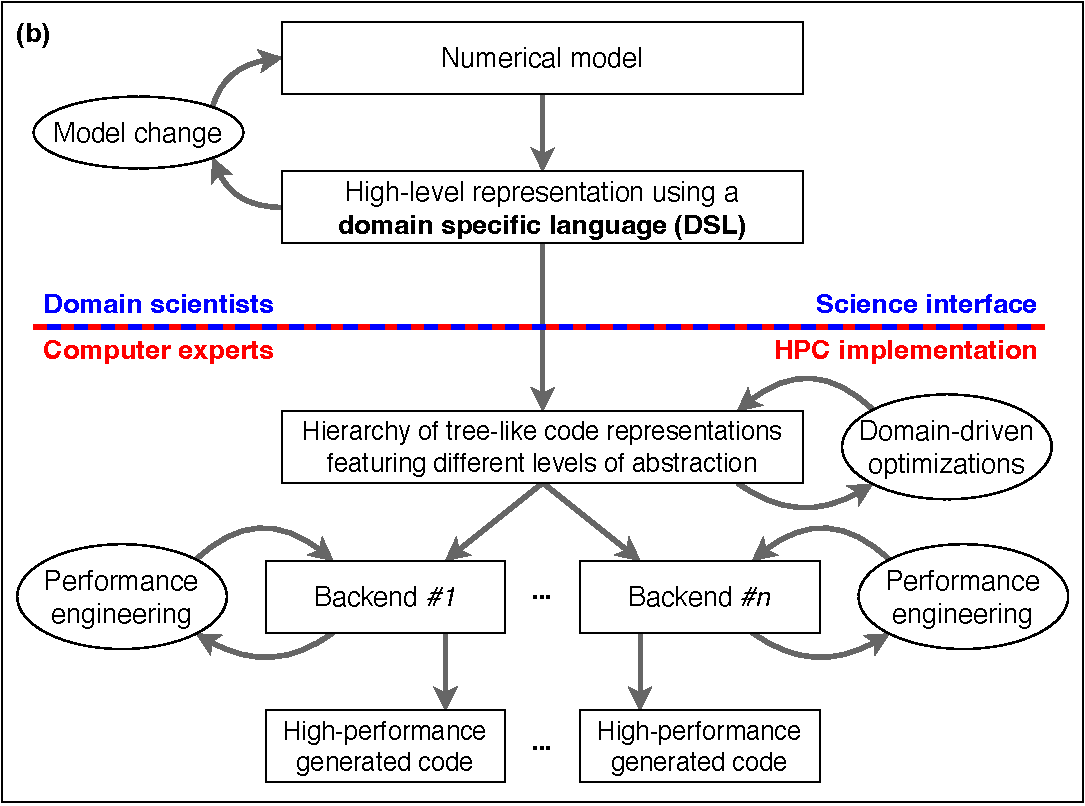
\includegraphics[scale=0.475]{workflow_dsl_2.pdf}
            \end{minipage}

            \caption{Diagrams comparing \textbf{(a)} a well-established workflow in scientific software development, and \textbf{(b)} a DSL-based approach resembling the software engineering strategy advocated in this paper. The red-and-blue dashed line in \textbf{(b)} mark the separation-of-concerns between the domain scientists and the computer experts.}
            \label{fig:dsl}
        \end{figure}

    \subsection{The GT4Py framework}
    \label{section:gt4py}

        GT4Py\footnote{\url{https://github.com/GridTools/gt4py}} is a Python library to generate high-performance implementations of stencil\footnote{A \emph{stencil} is an operator that computes array elements by accessing a fixed pattern of neighbouring items.} kernels as found in weather and climate applications. The library is developed and maintained by the Swiss National Supercomputing Center (CSCS), ETH Zurich, and the Swiss Federal Office of Meteorology and Climatology (MeteoSwiss), and benefits from important contributions by international partners such as the Paul Allen Institute for Artificial Intelligence (AI\textsuperscript{2}). The choice of embedding the GT4Py framework in Python has been mainly dictated by the following factors: (i) Python is taught in many academic courses due its clean, intuitive and expressive syntax, so that a significant fraction of early-career domain scientists \review{are} exposed to the language; (ii) it admits a powerful ecosystem of open source packages for building end-to-end applications; (iii) it is possible to seamlessly interface Python with lower-level languages with minimal overhead and virtually no memory copies; (iv) under the thrust of the Artificial Intelligence and Machine Learning community (AI/ML), the popularity and adoption of Python across the whole scientific community is constantly growing, as opposed to Fortran \citep{shipman23}. The proposed Python implementations of CLOUDSC and CLOUDSC2 are based on the first public release of GT4Py, which only supports Cartesian grids. Latest advancements to support unstructured meshes (contained in the sub-package \pyinline{gt4py.next}) are not discussed in this study.

        \begin{figure}[t!]
            \centering
            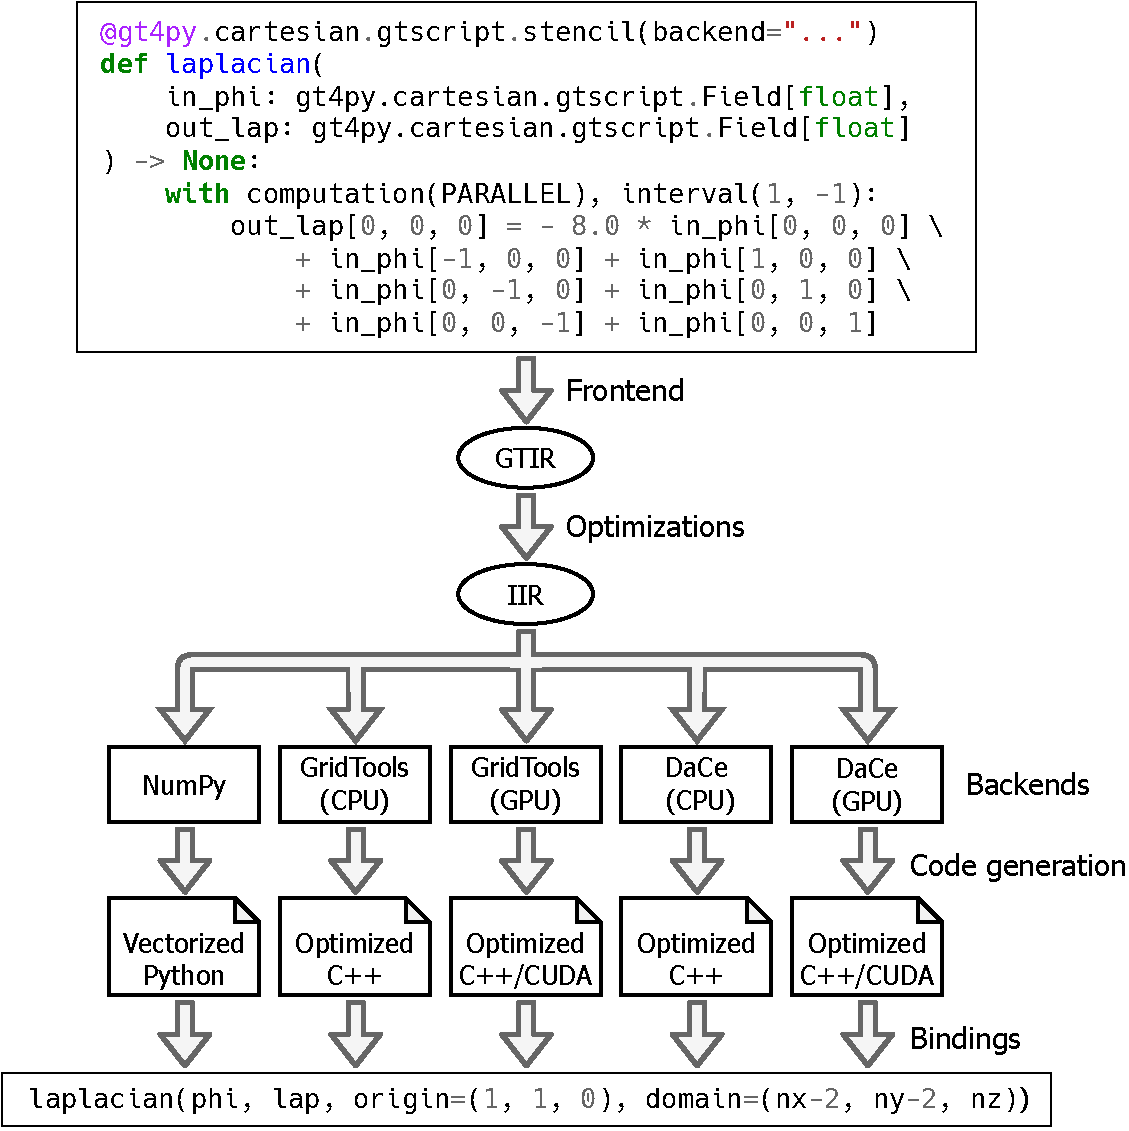
\includegraphics[scale=0.5]{gt4py_3.pdf}
            \caption{Simplified view on the internal stages carried out by the GT4Py toolchain to generate a high-performance CPU or GPU implementation of the \review{three-dimensional} Laplacian stencil starting from its GTScript definition. For the sake of visualization, only two intermediate representations (IRs) are included: the GridTools IR (GTIR) and the Implementation IR (IIR). }
            \label{fig:gt4py}
        \end{figure}

        Figure \ref{fig:gt4py} showcases the main steps undertaken by the GT4Py toolchain to translate the high-level definition of the horizontal Laplacian operator into optimized code, which can be directly called from within Python. The stencil definition is given as a regular Python function using the GTScript DSL. GTScript abstracts \review{spatial} for-loops away: computations are described for a single point of a three-dimensional Cartesian grid, and can be \review{diversified} for the vertical boundaries using the \pyinline{interval} context manager. Vertical loops are replaced by \pyinline{computation} contexts, which define the iteration order along the vertical axis: either \pyinline{PARALLEL} (meaning no vertical data dependencies between horizontal planes), \pyinline{FORWARD} or \pyinline{BACKWARD}. Each assignment statement within a computation block can be thought of as a loop over a horizontal plane; no horizontal data dependencies are allowed. Neighbouring points are accessed through relative offsets, with the first two offsets being the horizontal offsets, and the last offset being the vertical offset.

        Any function marked with the \pyinline{gt4py.cartesian.gtscript.stencil} decorator is translated by the GT4Py \emph{frontend} into a hierarchy of tree-like Intermediate Representations (IRs), featuring different levels of abstractions to accommodate diverse optimizations and transformations \citep{gysi21}. The lowest-level IR (denoted as Implementation IR, or IIR) is consumed by the \emph{backends} to generate code that is either optimized for a given architecture or suited to a specific purpose. The following backends are currently available:
        \begin{itemize}
            \item NumPy \citep{harris20} is the \emph{de facto} standard for array computing in Python, and can be used for debugging and fast-prototyping;
            \item GridTools \citep{afanasyev21} is a set of libraries and utilities to write performance-portable applications in the area of weather and climate;
            \item DaCe \citep{ben-nun19} is a parallel programming framework, which internally uses the Stateful DataFlow multiGraph (SDFG) data-centric intermediate representation to decouple domain science and performance engineering.
        \end{itemize}
        The generated code is compiled under the hood, and Python bindings for the resulting executable are automatically produced, so that the stencil can finally be executed by passing the input and output fields and by specifying the origin and size of the computation domain. GT4Py provides convenient utilities to allocate arrays with an optimal memory layout for any given backend, relying on NumPy for CPU storages and CuPy \citep{nishino17} for GPU storages. Concerning GPU computing, we highlight that GT4Py supports both NVIDIA and AMD GPUs.

        A more realistic and pertinent code sample is provided in Listing \ref{lst:saturation-stencil}. It is an abridged GT4Py implementation of the procedure computing the saturation water vapor pressure as a function of air pressure and temperature. The code is extracted from the CLOUDSC2-GT4Py dwarf and highlights two additional features of GTScript: functions and external symbols. Functions can be thought of as macros, and can be used to improve composability, reusability and readability. External symbols are used to encode those scalar parameters (e.g. physical constants) that are kept constant throughout a simulation, and might only change between different model setups. External values must be provided at stencil compilation time. The functionalities provided by the package \pyinline{ifs_physics_common} will be discussed in the following section.

        \begin{listing}[t!]
            \begin{minted}{py}
@gt4py.cartesian.gtscript.function
def foealfa(t):
    from __externals__ import RTICE, RTWAT, RTWAT_RTICE_R
    return min(1.0, ((max(RTICE, min(RTWAT, t)) - RTICE) * RTWAT_RTICE_R) ** 2.0)

@gt4py.cartesian.gtscript.function
def foeewmcu(t):
    from __externals__ import R2ES, R3IES, R3LES, R4IES, R4LES, RTT
    return R2ES * (
        foealfcu(t) * exp(R3LES * (t - RTT) / (t - R4LES))
        + (1.0 - foealfcu(t)) * (exp(R3IES * (t - RTT) / (t - R4IES)))
    )

@ifs_physics_common.framework.stencil.stencil_collection("saturation")
def saturation(
    in_ap: gtscript.Field[float], in_t: gtscript.Field[float], out_qsat: gtscript.Field[float]
):
    from __externals__ import LPHYLIN, QMAX, R2ES, R3IES, R3LES, R4IES, R4LES, RETV, RTT
    with computation(PARALLEL), interval(...):
        if LPHYLIN:  # linearized physics
            alfa = foealfa(in_t)
            foeewl = R2ES * exp(R3LES * (in_t - RTT) / (in_t - R4LES))
            foeewi = R2ES * exp(R3IES * (in_t - RTT) / (in_t - R4IES))
            foeew = alfa * foeewl + (1.0 - alfa) * foeewi
            qs = min(foeew / in_ap, QMAX)
        else:
            ew = foeewmcu(in_t)
            qs = min(ew / in_ap, QMAX)
        out_qsat[0, 0, 0] = qs / (1.0 - RETV * qs)
            \end{minted}

            \caption{GTScript (the Python-embedded DSL exposed by GT4Py) functions and stencil computing the saturation water vapor pressure given the air pressure and temperature. Abridged excerpt from the CLOUDSC2-GT4Py dwarf.}
            \label{lst:saturation-stencil}
        \end{listing}

    %\biblio
\end{document}
